\documentclass[a4paper,11pt,final]{article}
\usepackage{fancyvrb, color, graphicx, hyperref, amsmath, url}
\usepackage{palatino}
\usepackage{pygments}
\usepackage[a4paper,text={16.5cm,25.2cm},centering]{geometry}
        
\hypersetup  
{   pdfauthor = {Maria Eduarda Bicalho},
  pdftitle={FIR filter design with Python and SciPy},
  colorlinks=TRUE,
  linkcolor=black,
  citecolor=blue,
  urlcolor=blue
}

\setlength{\parindent}{0pt}
\setlength{\parskip}{1.2ex}

        
\title{Relatório Intermediário}
\author{Maria Eduarda Bicalho}
\date{30 de abril de 2020}

\begin{document}
\maketitle

\section{Descrição do Problema}

    O projeto Maximin Share tem como objetivo fazer a divisão mais justa possível de um número de objetos com 
diferentes valores entre um número diferente de pessoas. O problema pincipal se centra em como realizar 
essa divisão. Dessa forma, três diferentes técnicas -  Herística, Busca Local e Busca Global - foram utilizadas 
para produzir três diferentes algoritmos para executar essa partição.
    Neste relatório essas três implementções serão analisadas com diferentes entradas para avaliar as
alterções em suas saídas. Essas entradas possuírão diferentes tamanhos, alterando significamente. 
Primeiramente, em relação a quantidade de pessoas e depois a quantidade de objetos. Dentro de cada uma dessas 
análises, serão estudados o tempo, e a qualidade da solução em relação aos diferentes dimensões de entradas.
A qualidade será analisada apartir do MMS (o valor da pessoa com o menor valor), ou seja quanto maior o MMS 
maior a qualidade da saída.


\subsection{Máquina utilizada}

Memória :  1.5 GiB  -
  Disco : 63 GB  -
  Processador : Intel i5 -
  Virtualização: KVM  -


\section{Efeito número de pessoas}

   Nessa seção será realizada a análise do impacto de uma entrada com diferentes números de pessoas
nos 3 diferentes algoritmos implementados no projeto.A capacidade da máquina foi sendo testada,
aumentando cada vez mais o input de com o número pessoas. A variação do número de objetos foi baixa,
para que a mudança dessa variável não fosse importante para o tempo e qualidade da solução, e esses 
se mantivessem em função do delta pessoas. A busca global não conseguiu um tempo factível depois 
de um número de entrada de 10 pessoas, dessa forma, esse algoritmo aparecerá somente até o valor 
de entrada 10 - para as demais entradas foi assumido um valor limite. 




\subsection{Tempo}

Nesta seção, a medida utilizada para a análise será a do tempo.





\begin{verbatim}
<matplotlib.legend.Legend at 0x7f3d2cc46cd0>
\end{verbatim}
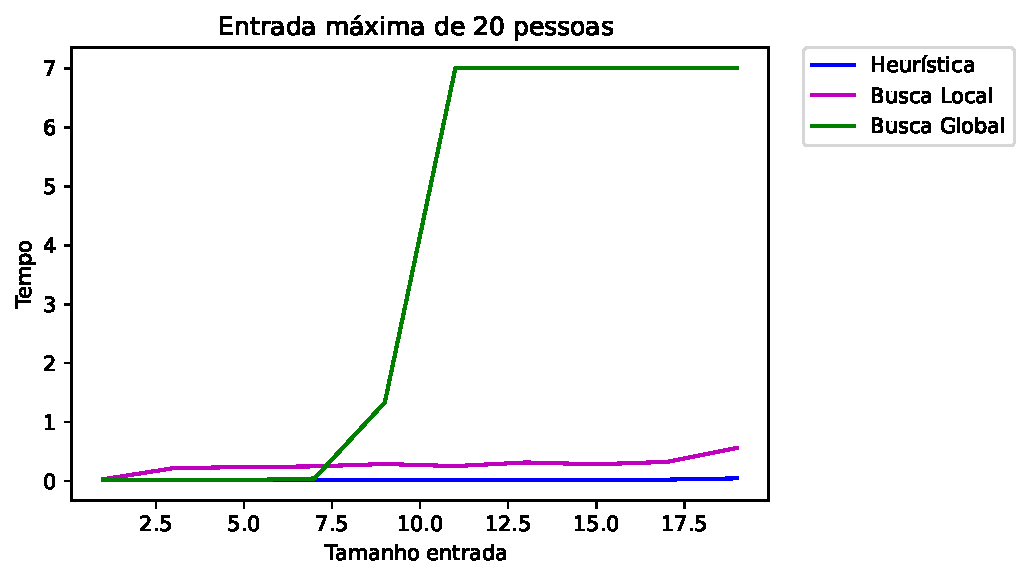
\includegraphics[width= 15 cm]{figures/teste_figure3_1.pdf}


\begin{verbatim}
<matplotlib.legend.Legend at 0x7f3d2cad9ca0>
\end{verbatim}
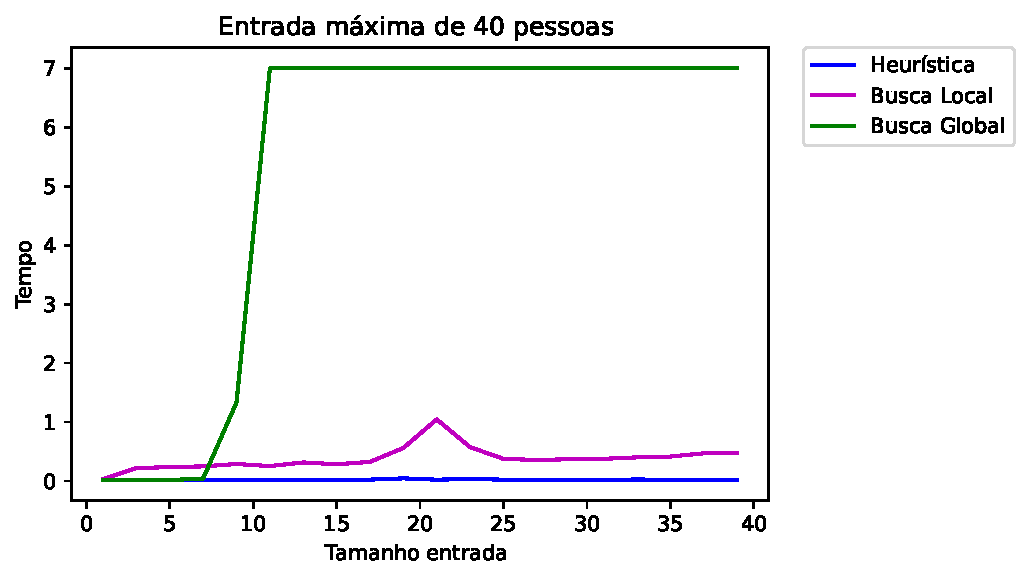
\includegraphics[width= 15 cm]{figures/teste_figure4_1.pdf}



\begin{verbatim}
<matplotlib.legend.Legend at 0x7f3d2c9fa5b0>
\end{verbatim}
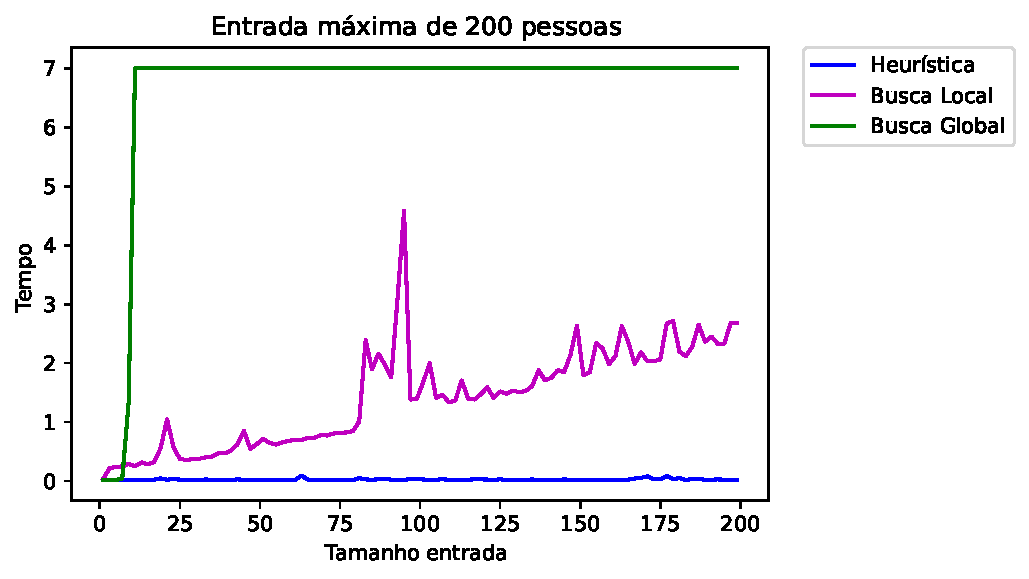
\includegraphics[width= 15 cm]{figures/teste_figure5_1.pdf}


A partir dos gráficos pode-se concluir que os algoritmos de busca local de busca global possuem 
valores de tempo maiores do que a heurística, a qual não sofre fortes alterações. Um fato curioso que pode ser
observado é que a busca local inicia com um tempo maior e logo antes da entrada de 10  - por volta da entrada de 7- 
é ultrapassada rapidamente pela busca global, cuja variação é extremamente alta. Por realizar a busca no resultado 
apresentado e não em todos os possíveis, a busca local já possui um tempo maior, mas factível na máquina utilizada 
e possi um resultado melhor que o da heurística.Por ser um algoritmo que utiliza.recursão e percorre todos 
os caminhos possíveis para certificar que possui o melhor, a implementação da busca global
cresce rapidamente. O único esforço da solução heuristíca é o de ordenar, por isso o tempo não sofre grandes alterações.

\subsection{Qualidade da solução}


\begin{verbatim}
<matplotlib.legend.Legend at 0x7f3d2c97bfa0>
\end{verbatim}
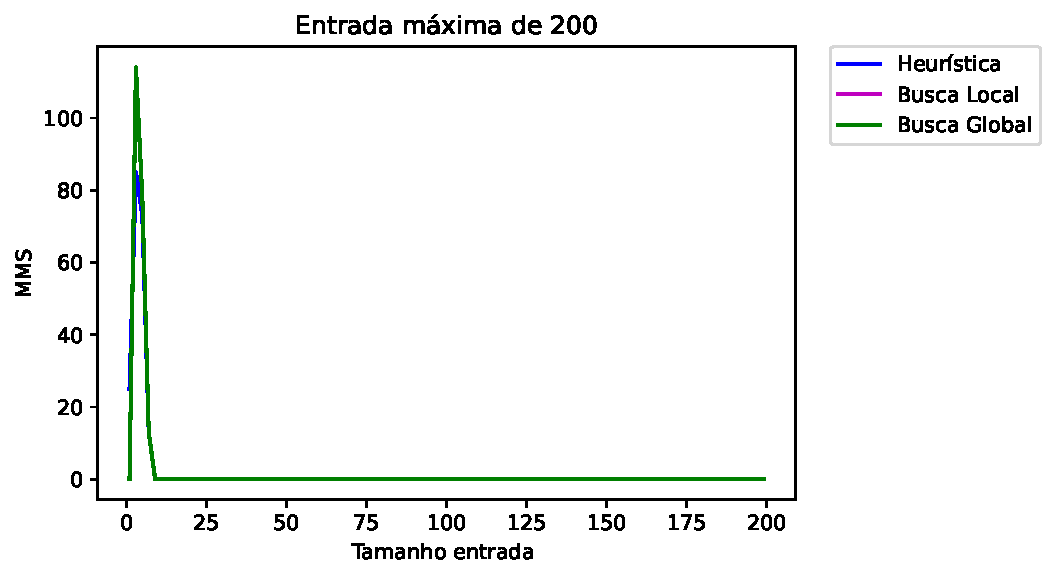
\includegraphics[width= 15 cm]{figures/teste_figure6_1.pdf}


A análise da qualidade da solução com um aumento significativo no número de pessoas com uma mudança pequena
na quantidade de objetos não é muito eficiciente, pois em determinado valor, não terá objetos suficientes 
para a quantidade de pessoas. Dessa forma somente entradas bem pequenas são avaliadas. Todavia, mesmo com 
essa restrição já é possível analisar que o resultado da busca global e da busca local possui um maior 
qualidade do que o da heurística. 

\section{Efeito número de objetos}

Nessa seção será realizada a análise do impacto de uma entrada com diferentes números de objetos
nos 3 diferentes algoritmos implementados no projeto. A capacidade da máquina foi sendo testada,
aumentando cada vez mais o input de com o número objetos. A variação do número de pessoas foi baixa,
para que a mudança dessa variável não fosse importante para o tempo e qualidade da solução, e esses 
se mantivessem em função do delta objetos. A busca global não conseguiu um tempo factível depois 
de um número de entrada de 10 pessoas. Dessa forma, esse algoritmo aparecerá somente até o valor 
de entrada 10 - para as demais entradas foi assumido um valor limite. 




\subsection{Tempo}

Nesta seção, a medida utilizada para a análise será a do tempo.








\begin{verbatim}
<matplotlib.legend.Legend at 0x7f3d2c9013a0>
\end{verbatim}
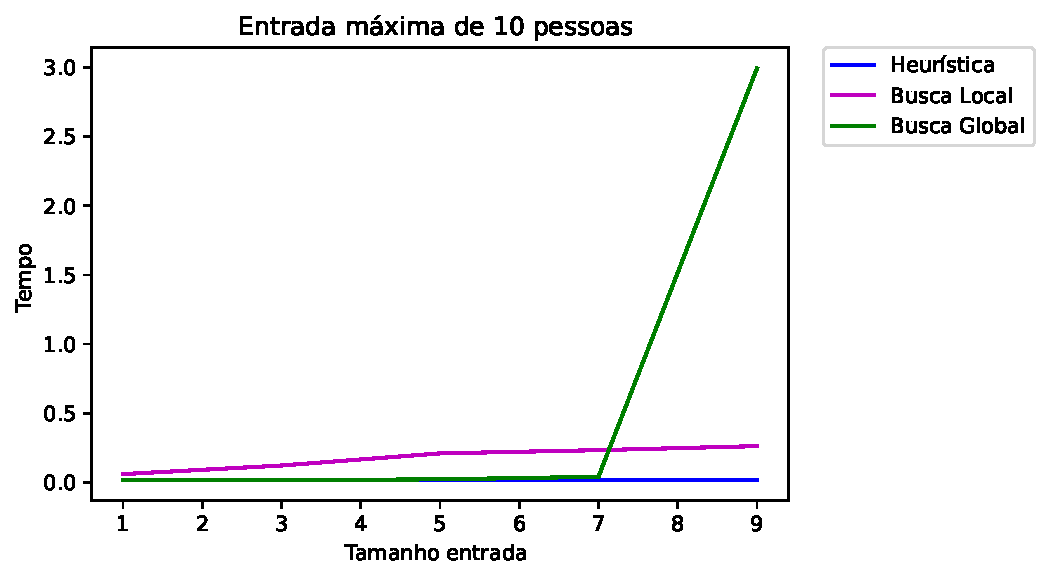
\includegraphics[width= 15 cm]{figures/teste_figure10_1.pdf}



\begin{verbatim}
<matplotlib.legend.Legend at 0x7f3d2c83c970>
\end{verbatim}
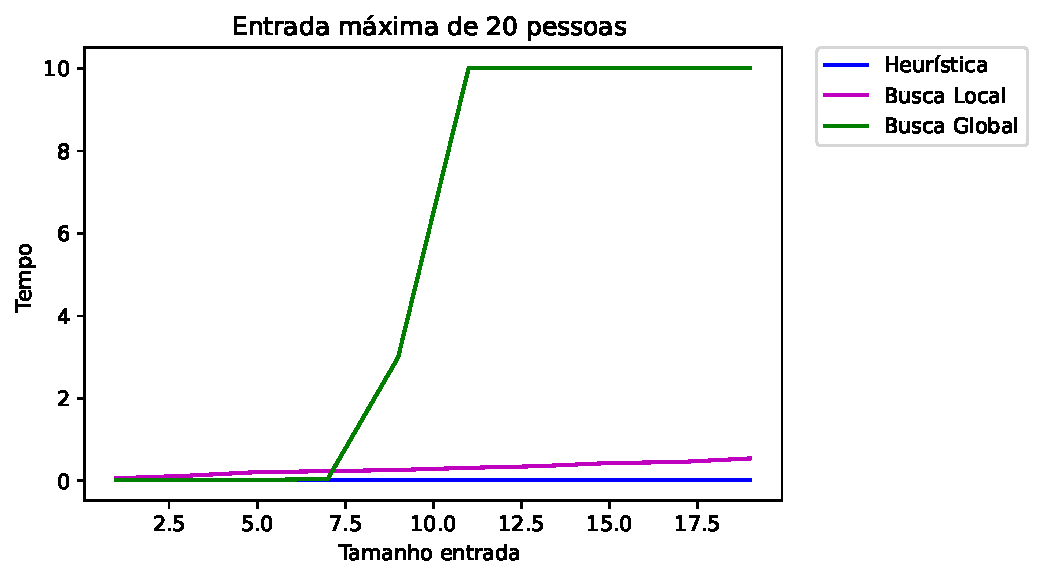
\includegraphics[width= 15 cm]{figures/teste_figure11_1.pdf}



\begin{verbatim}
<matplotlib.legend.Legend at 0x7f3d2ca538e0>
\end{verbatim}
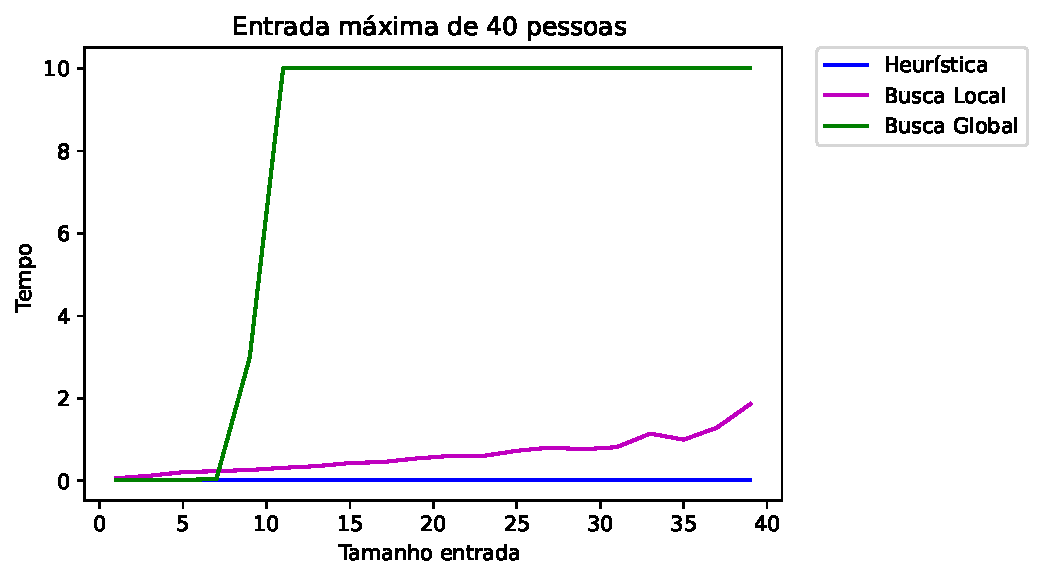
\includegraphics[width= 15 cm]{figures/teste_figure12_1.pdf}



\begin{verbatim}
<matplotlib.legend.Legend at 0x7f3d2cc27430>
\end{verbatim}
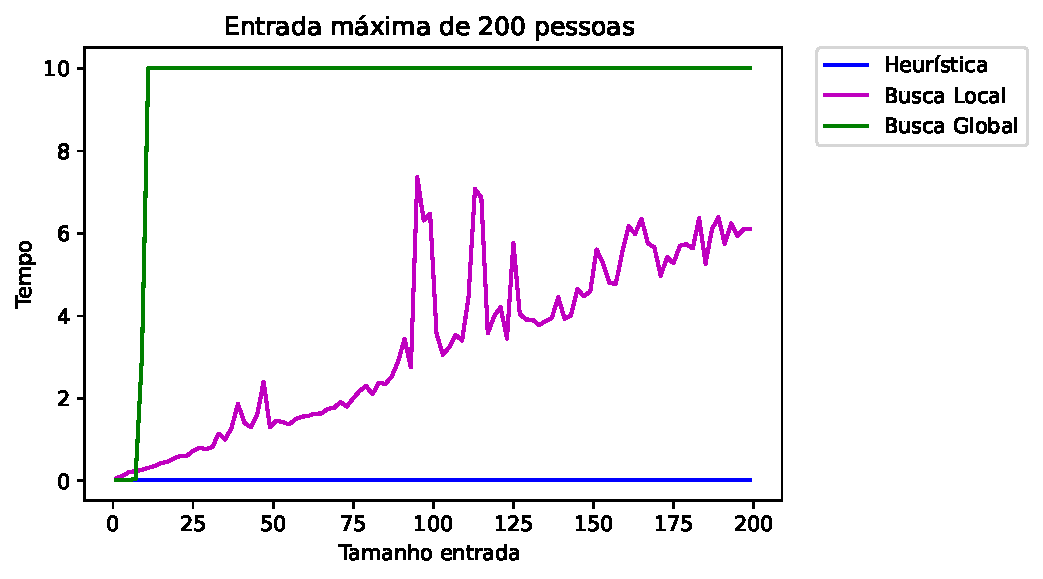
\includegraphics[width= 15 cm]{figures/teste_figure13_1.pdf}



Como analisado no gráfico do tempo da seção anterior, a busca local e a busca global possuem uma 
variação significamente maior do que a heurística. Nas entradas pequenas as 3 implementações possuem 
tempos parecidos, mas há uma relação direta com o aumento da quantidade de objetos na entrada e com a
aumento do tempo da busca global e local, enquanto o tempo da heurística não altera muito. Novamente
é perceptível a rápida mudança no tempo da busca global, que inicia inferior ao da busca local e depois
aumenta drasticamente.

\subsection{Qualidade da solução}


\subsubsection{Gráficos}


\begin{verbatim}
<matplotlib.legend.Legend at 0x7f3d2ca42d30>
\end{verbatim}
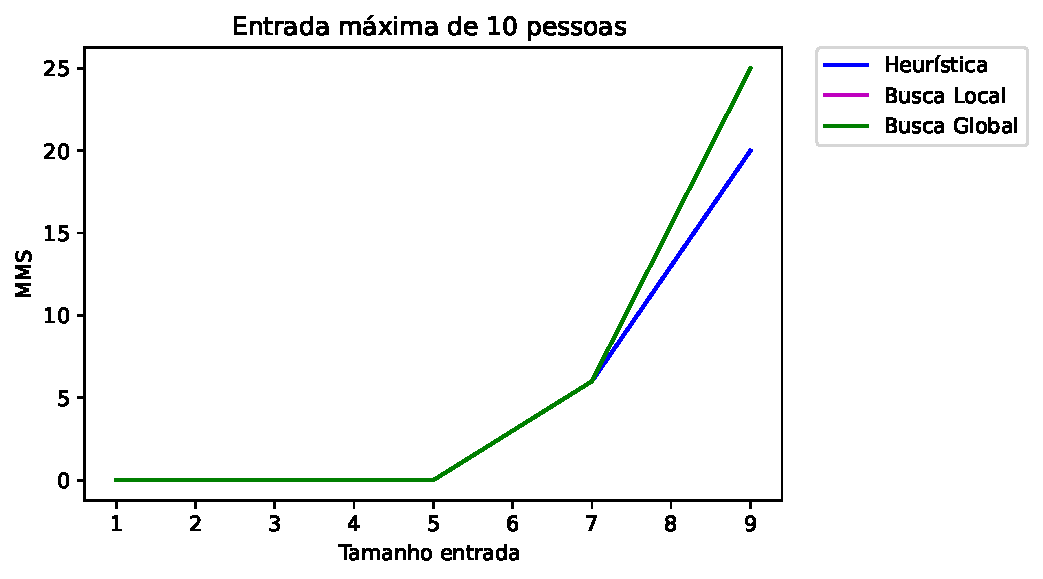
\includegraphics[width= 15 cm]{figures/teste_figure14_1.pdf}



\begin{verbatim}
<matplotlib.legend.Legend at 0x7f3d2cac6190>
\end{verbatim}
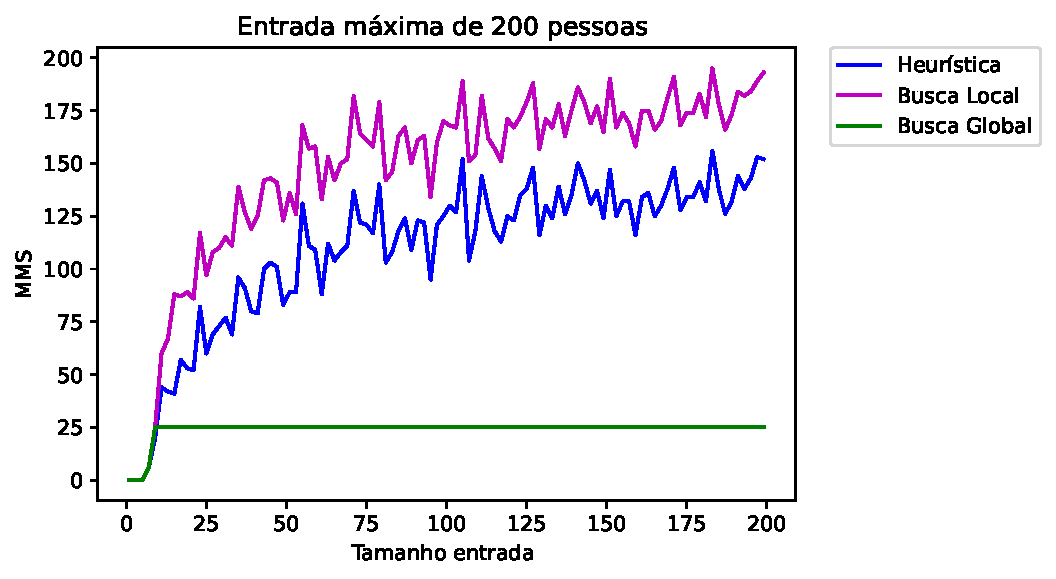
\includegraphics[width= 15 cm]{figures/teste_figure15_1.pdf}


No último gráfico de qualidade da solução pode ser observado que com entradas pequenas os três algoritmos 
possuem resultados parecido. Contanto, com o aumento do número de objetos a diferença entre a busca local
heurística vai se tornando cada vez maior. No priemiro gráfico de qualidade da solução pode ser observado 
que a busca global estava crescendo com variação parecida da busca local, ou seja, pode se que
essas duas implementacões, se possível avaliar, tivessem resultados mais parecidos do que os da 
busca local e da heurística.


\section{Conclusão}

As implentações analisadas no relatório possuem algumas caracteristicas diferentes. Para entradas pequenas 
os algoritmos apresentam soluções com qualidades muito parecidas, e o tempo da heurística 
já inicia um pouco menor. Dessa forma essa algoritmo parece ser eficiente para entradas pequenas, 
uma vez que é mais rápido e possui saídas com alta qualidade. Na medida que o a entrada aumenta o tempo da
busca local e global aumenta, e a qualidade da solução da heurística cai. Assim sendo, para entradas cada vez
maiores, resultados cada vez maiores são tidos a partir da busca local. Consequentemente, as implementações 
podem ser utilizadas para diferentes finalidades, cada uma podendo ser escolhida a partir das preferências e 
importâncias de determinado projeto.



\end{document}
